\subsection{Maximum Growth Rate is Determined by the Ribosomal Mass Fraction}
\label{sec:limit}
The 7 minute speed limit shown in Figure \ref{fig:protein_synthesis}(B) assumes all
proteins in the cell are ribosomes. In order to connect this to the
experimental data (and physiological reality more broadly), we first need to relax this assumption and determine a
translation-limited growth rate. Here, we will assume that the cell is composed
of $N_\text{pep}$ peptide bonds and $R$ ribosomes, whose precise values will depend on the
growth rate $\lambda$. The protein subunits of each ribosomal protein sum to a
total of $\approx$ 7500 amino acids as noted earlier, which we denote by $L_R$.
With an average mass of an amino acid of $m_\text{AA} \approx$ 110
Da (BNID: 104877), the total ribosomal mass fraction  $\Phi_R$ is given by
\begin{equation}
  \Phi_R = \frac{m_\text{ribosomes} }{m_\text{proteome}} \approx \frac{m_\text{AA} \times R \times L_R}{m_\text{AA} \times N_\text{pep}} = \frac{R \times L_R}{N_\text{pep}}.
  \label{eq:phir}
\end{equation}
For exponentially growing cells \citep{godin2010}, the rate of cellular growth will
be related to the rate of protein synthesis via
\begin{equation}
  \lambda N_\text{pep} = r_t \times R \times f_a,
  \label{eq:lam_npep}
\end{equation}
where $r_t$ is the translation rate. Here, we've introduced a multiplicative
factor $f_a$ which represents the fraction of the ribosomes that are actively
translating. This term allows us to account for immature or
non-functional ribosomes or active sequestration of ribosomes through the action
of the secondary messenger alarmone (p)ppGpp in poorer nutrient conditions \citep{hauryliuk2015}.

Combining Equation \ref{eq:phir} and Equation \ref{eq:lam_npep} results in an expression for a
translation-limited growth rate, which is given by
\begin{equation}
\lambda_\text{translation-limited} = \frac{r_t\times \Phi_R\times f_a}{L_R}.
\label{eq:lam_limited}
\end{equation}
This result, derived in a similar manner by others \citep{dennis2004, klumpp2013}, reflects
mass-balance under steady state growth and has long provided a rationalization
of the apparent linear increase in \textit{E. coli}'s ribosomal content as a
function of growth rate \citep{goldberger1979, dennis2004, scott2010, dai2016}. The
left-hand panel of Figure \ref{fig:ribosome_limit}(A) shows this growth rate plotted as a
function of the ribosomal mass fraction.  In the regime where all ribosomes are
active ($f_a = 1$) and the entire proteome is composed of ribosomal proteins
($\Phi_R = 1$), indeed, we arrive at the maximum theoretical growth rate of $r_t
/ L_R$, and $\approx$ 7 min for \textit{E. coli}.

Connecting Equation \ref{eq:lam_limited} to the proteomic data, however, requires knowledge of $f_a$ at each growth rate as proteomic
measurements only provide a measure of $\Phi_R$. Recently, \cite{dai2016}
determined $f_a$ as a function of the growth rate (Figure \ref{fig:ribosome_limit}(A),
right-hand panel, inset), revealing that $f_a \approx 1$ at growth rates above
0.75 hr$^{-1}$ and $f_a < 1$ at slower growth rates. Using these data, we
inferred the approximate active fraction (see the Appendix Section "Calculation
of active ribosomal fraction") at each growth rate and used this to compute
$\Phi_R \times f_a$ (Figure \ref{fig:ribosome_limit}(A), colored points in right-hand
panel). Importantly, these data largely skirt the translation-limited growth rate
determined using Equation \ref{eq:lam_limited}, where we have taken $r_t$ to be the maximal
elongation rate of 17 amino acids per second measured by \cite{dai2016}. There
is a notable discrepancy between the data collected in \cite{schmidt2016,
li2014} and that collected from \cite{valgepea2013, peebo2015}. When compared to
other measurements (non-proteomic based) of the active ribosome mass fraction
based on measurements of total RNA to total protein mass ratios
(Figure \ref{fig:ribosome_limit}(B), grey points in right-hand panel and  further detailed
in Figure \ref{fig:ribosome_limit_supp}), the data from
\cite{valgepea2013} and \cite{peebo2015} are notably different, suggesting there
may be a systematic bias in these two sets of measurements.

Together, these results illustrate that the growth rates observed across the
amalgamated data sets are indeed close to the translation-limited growth rate
set by ribosomal activity, at least for the data reported in \cite{schmidt2016}
and \cite{li2014}. While this is a useful framework to consider how the relative
abundance of ribosomes (compared to all other proteins) defines the growth rate,
it is worth noting that as growth rate increases, so does the cell size and
therefore so will the total proteomic mass \citep{basan2015}. With a handle on
how elongation rate and the total number of peptide bonds per proteome is
related to the growth rate, we now expand this description to account for the
increasing chromosomal content, cell size, and  ribosome copy number at faster
growth rates, enabling us to identify a potential bottleneck in the synthesis of
rRNA.

\begin{figure}
        \centering{
        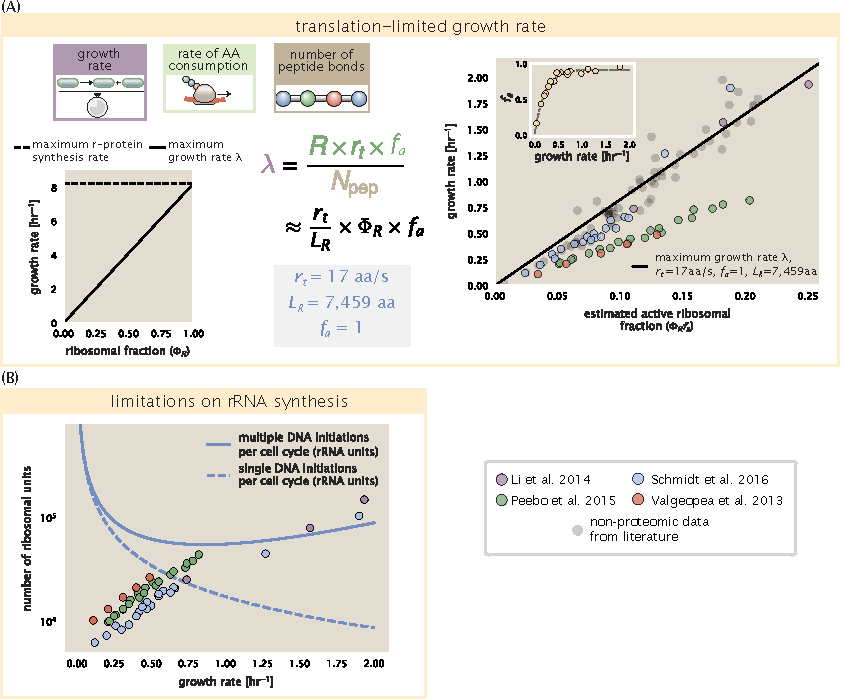
\includegraphics{main_figs/fig10_ribosome_as_limit.pdf}
        \caption{\textbf{Translation-limited growth rate.}  (A) \textit{left}:
        Translation-limited growth as a function of the ribosomal fraction. The
        solid line is calculated for an elongation rate of 17 aa per second.
        The dashed line corresponds to the maximum rate of ribosomal protein
        synthesis ($\approx$ 7 min).
        \textit{right}: Translation-limited growth rate as a function of the actively translating ribosomal fraction.
        The actively translating ribosomal fraction is calculated using the
        estimated values of $f_a$ from  \cite{dai2016} (shown in inset; see
         Section "Calculation of active ribosomal fraction" for additional detail). Gray data points
        show additional measurements from literature and considered further in
        the supplemental figure part (A).
        (B) Maximum number of
        rRNA units that can be synthesized as a function of growth rate.
        Solid curve corresponding to the rRNA copy number is calculated by
        multipyling the number of rRNA operons by the estimated number of
        $\langle\text{\# ori}\rangle$ at each growth rate. The quantity
        $\langle\text{\# ori}\rangle$ was calculated using Equation 4 and
        the measurements from \cite{si2017}. The dashed line shows the maximal
        number of functional rRNA units produced from a single chromosomal
        initiation per cell cycle. } \label{fig:ribosome_limit}}
\end{figure}

\subsection{rRNA Synthesis Presents a Potential Bottleneck During Rapid Growth}
Even under idealized experimental conditions, \textit{E. coli} rarely
exhibits growth rates above 2 hr$^{-1}$ \citep{bremer2008}, which is still
well-below the synthesis rate of a single ribosome, and below the maximum
growth rates reported for several other bacteria \citep{roller2016}. While we
have considered potential limits imposed by translation of ribosomal
\textit{proteins}, here we consider potential limiting regimes specific to the
synthesis of rRNA.

Due to multiple initiations of chromosomal replication per cell doubling, the
effective number of rRNA operons increases with growth rate and will do so in
proportion to the average number of chromosomal origins per cell, $\langle$\# ori$\rangle$.
This later parameter is set by how often replication must be initiated in order
to keep up with the cell doubling time $\tau$, whose time may be shorter than the
cell cycle time $\tau_{cyc}$ (referring to the time from replication initiation to
cell division) \citep{dennis2004, ho2015}. This is quantified by
\begin{equation}
    \langle \text{\# ori} \rangle = 2^{\tau_{cyc} / \tau} = 2^{\tau_{cyc} \lambda / \log(2)},
    \label{eq:Nori}
\end{equation}
where the doubling time $\tau$ is related to the growth rate by $\tau =
\log(2)/\lambda$. As the rRNA operons are predominantly located close to the
origin of replication (BNID: 100352), we make the simplifying assumption that
that the number of rRNA operons will be directly proportional to $\langle$\#
ori$\rangle$.  We used the experimental measurements of $\tau_{cyc}$ (the
timescale of chromosome replication and cell division) and $\tau$ (the timescale
of a cell doubling)  [Figure \ref{fig:ribosome_limit_supp}(B)] to
calculate $\langle$\# ori$\rangle$  with Equation \ref{eq:Nori} as a function of growth
rates. For growth rates above about 0.5 hr$^{-1}$, $t_{cyc}$ is approximately
constant at about 70 minutes, implying an exponential increase in $\langle$\# ori$\rangle$  and
the rRNA operon copy number for growth rates above 0.5 hr$^{-1}$.

Returning to our rule-of-thumb that one functional rRNA unit is produced per
second per transcribing operon, we can estimate the maximum number of ribosomes
that could be made as a function of growth rate (Figure \ref{fig:ribosome_limit}(B), blue
curve). Although we expect this estimate to significantly overestimate rRNA
abundance at slower growth rates ($\lambda < 0.5\, \text{hr}^{-1}$), this
provides a useful reference alongside the proteomic measurements, particularly
in the regime of fast growth. For growth rates above about 1 hr$^{-1}$ in
particular, we find that cells will need to transcribe rRNA near their maximal
rate. As a counter example, if \textit{E. coli} did not initiate multiple rounds
of replication, but could still replicate their chromosome within the requisite
time limit, they would be unable to make enough rRNA for the observed number of
ribosomes (dashed blue curve in Figure \ref{fig:ribosome_limit}(C)). The convergence
between the maximum rRNA production and measured ribosome copy number suggests
rRNA synthesis may begin to present a bottleneck at the fastest growth rates in
\textit{E. coli} due to the still-limited copies of rRNA genes.
